\begin{figure}[htbp]
    \centering
    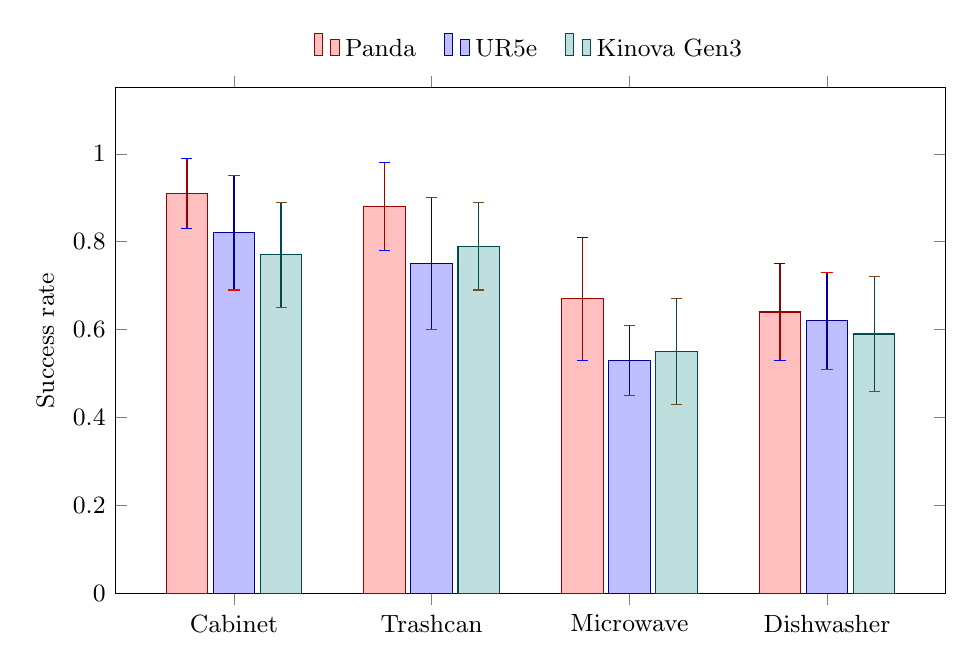
\begin{tikzpicture}
    \begin{axis}[
        ybar=2pt,
        bar width=15pt,
        width=\textwidth, height=8cm,
        enlarge x limits=0.2,
        ymin=0, ymax=1.15,
        ylabel={Success rate},
        symbolic x coords={Cabinet, Trashcan, Microwave, Dishwasher},
        xtick={Cabinet, Trashcan, Microwave, Dishwasher},
        legend style={at={(0.5,1.03)}, anchor=south, legend columns=3,
                      font=\small, draw=none, /tikz/every even column/.append style={column sep=8pt}},
        error bars/y dir=both, error bars/y explicit,
        tick label style={font=\small},
        label style={font=\small},
    ]
    % Panda
    \addplot+[draw=red!60!black, fill=red!25] coordinates {
        (Cabinet,0.91) +- (0,0.08) (Trashcan,0.88) +- (0,0.10)
        (Microwave,0.67) +- (0,0.14) (Dishwasher,0.64) +- (0,0.11) };
    % UR5e
    \addplot+[draw=blue!60!black, fill=blue!25] coordinates {
        (Cabinet,0.82) +- (0,0.13) (Trashcan,0.75) +- (0,0.15)
        (Microwave,0.53) +- (0,0.08) (Dishwasher,0.62) +- (0,0.11) };
    % Kinova Gen3
    \addplot+[draw=teal!60!black, fill=teal!25] coordinates {
        (Cabinet,0.77) +- (0,0.12) (Trashcan,0.79) +- (0,0.10)
        (Microwave,0.55) +- (0,0.12) (Dishwasher,0.59) +- (0,0.13) };
    \legend{Panda, UR5e, Kinova Gen3}
    \end{axis}
    \end{tikzpicture}
    \caption[Cross-robot transfer with \FLEX{}]{Bar-chart visualization of the cross-robot transfer results reported in \cref{tab:flex_transfer}. The same learned policies are deployed on three robot platforms without retraining; error bars denote one standard deviation. Performance remains consistent across embodiments, demonstrating that the force-space representation enables direct embodiment transfer.}
    \label{fig:flex_transfer_bars}
\end{figure}
